\documentclass[11pt,a4paper,notitlepage,twocolumn]{article}

\usepackage[T1]{fontenc}
\usepackage[utf8]{inputenc}
\usepackage[english]{babel}
\usepackage{amsmath}
\usepackage{amsfonts}
\usepackage{amssymb}
\usepackage{verbatim}
\usepackage{listings}
\usepackage{color}
\usepackage{setspace}
\usepackage{epstopdf}
\usepackage{graphicx}
\usepackage{caption}
\usepackage{subcaption}
\usepackage{float}
\usepackage{epstopdf}
\usepackage{hyperref}
\usepackage{dsfont}
\usepackage{braket}
\pagenumbering{arabic}
\usepackage{tikz}
\usepackage{fullpage}
\usepackage{titling}

\definecolor{codepurple}{rgb}{0.58,0,0.82}
\definecolor{backcolour}{rgb}{0.95,0.95,0.92}
\definecolor{dkgreen}{rgb}{0,0.6,0}
\definecolor{gray}{rgb}{0.5,0.5,0.5}
\definecolor{mauve}{rgb}{0.58,0,0.82}
%\setlength{\parindent}{0pt}

\lstdefinestyle{pystyle}{
  language=Python,
  aboveskip=3mm,
  belowskip=3mm,
  columns=flexible,
  basicstyle={\small\ttfamily},
  backgroundcolor=\color{backcolour},
  commentstyle=\color{dkgreen},
  keywordstyle=\color{magenta},
  numberstyle=\tiny\color{gray},
  stringstyle=\color{codepurple},
  basicstyle=\footnotesize,  
  breakatwhitespace=false
  breaklines=true,
  captionpos=b,
  keepspaces=true,
  numbers=left,
  numbersep=5pt,
  showspaces=false,
  showstringspaces=false,
  showtabs=false,
  tabsize=2
}
\lstdefinestyle{iStyle}{
  language=IDL,
  aboveskip=3mm,
  belowskip=3mm,
  columns=flexible,
  basicstyle={\small\ttfamily},
  backgroundcolor=\color{backcolour},
  commentstyle=\color{dkgreen},
  keywordstyle=\color{magenta},
  numberstyle=\tiny\color{gray},
  stringstyle=\color{codepurple},
  basicstyle=\footnotesize,  
  breakatwhitespace=false
  breaklines=true,
  captionpos=b,
  keepspaces=true,
  numbers=left,
  numbersep=5pt,
  showspaces=false,
  showstringspaces=false,
  showtabs=false,
  tabsize=2
}
\lstdefinestyle{c++style}{
  language=C++,
  keywordstyle=\color{blue}\ttfamily,
  stringstyle=\color{red}\ttfamily,
  commentstyle=\color{green}\ttfamily,
  morecomment=[l][\color{magenta}]{\#}
  aboveskip=3mm,
  belowskip=3mm,
  columns=flexible,
  basicstyle={\small\ttfamily},
  backgroundcolor=\color{backcolour},
  numberstyle=\tiny\color{gray},
  basicstyle=\footnotesize,  
  breakatwhitespace=false
  breaklines=true,
  captionpos=b,
  keepspaces=true,
  numbers=left,
  numbersep=5pt,
  showspaces=false,
  showstringspaces=false,
  showtabs=false,
  tabsize=2
}
\newcommand{\SE}{Schr\"odinger equation}
\newcommand{\laplacian}{\vec{\nabla}^2}
\newcommand{\eye}{\mathds{I}}
\newcommand\pd[2]{\frac{\partial #1}{\partial #2}}
\def\doubleunderline#1{\underline{\underline{#1}}}


\title{\normalsize Fys3150/4150 - Computational Physics\\
\vspace{10mm}
\huge 5. Continuation on Astronomical project -\\ $N$-body simulation of an open galactic cluster\\
\vspace{10mm}
\normalsize Due date {\bf Nov 9$^{th}$, 2016}}

% Skriv namnet ditt her og fjern kommenteringa
\author{Magnus Christopher Bareid \\ un: magnucb }


\begin{document}
\vspace{5mm}

\begin{titlingpage}
	\begin{center}
    	
\includegraphics[scale=0.5]{../ITA_seal.png}
    	\let\newpage\relax\maketitle

		\begin{figure}[H]
		\center
		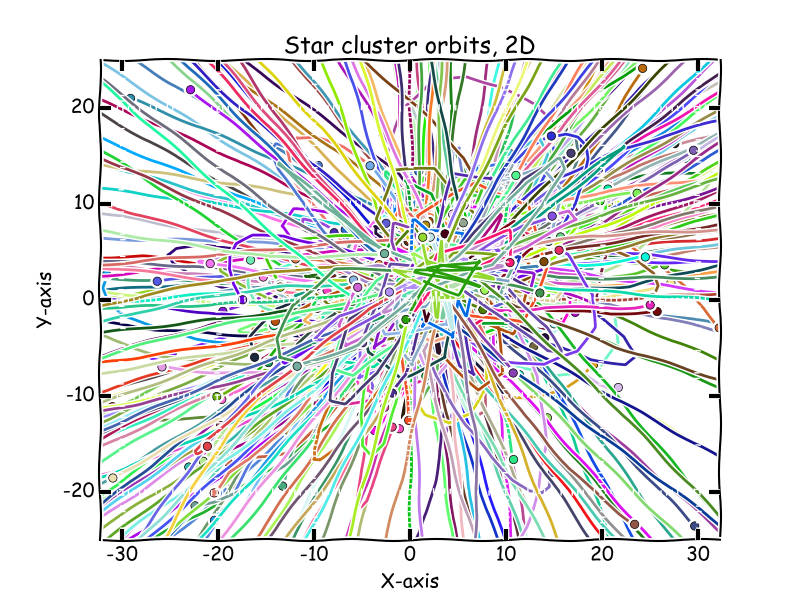
\includegraphics[scale=0.5]{../frontpage.png}
		\end{figure}

		\begin{abstract}
This project is a continuation on a previous project given to the students this semester, in which the students were to gravitationally and numerically simulate the Solar System.

For the current project, the students are to simulate an $N$-body system, unrelated to the Solar system, and investigate properties of the system as it is simulated to reflect on the model's physical validity.
		\end{abstract}

		\newpage
		\tableofcontents

	\end{center}
\end{titlingpage}

%\begin{center}
%\line(1,0){450}
%\end{center}


\newpage

\section*{N-body simulation of an open galactic cluster}
\section{Introduction}
For this project I will review the mathematical equations related to Newtonian gravitation and other relevant equations, in order to simulate a stellar $N$-body system that starts out motionless before it begins to collapse in on itself, a so-called \textit{cold collapse}.

It is worth noting that the differential integration method that I utilize is the Velocity Verlet method, as opposed to the Euler or RungeKutta4 method which were mentioned in the previous astronomical project.

The physical properties which I will investigate through this project are:
\begin{itemize}
\item energy conservation in an $N$-body system and its related equilibrium,
\item numerical instabilities from round-off corrections,
\item validity of the virial theorem,
\item radial distribution of stellar bodies in a gravitationally bound system.
\end{itemize}

\section{Underlying math}
The most important mathematical expression for an assignment investigating properties of a gravitational system, will be the equations gravitational force exchange.
\subsection{Newton's laws}
The force equation between two objects, will be as per Newton's law of gravity:
\begin{align}\label{eq:gravlaw}
\vec{F}_{G_{i,j}} &= -G\frac{m_i m_j}{r^3_{i,j}}\vec{r}_{i,j}
\end{align}
where $i$ and $j$ denotes which objects' force, in the system of objects' forces, are being measured, the $m$s represents their masses, $r$ is the displacement between the two objects, and $G$ is the Newton's gravitational constant.

Furthermore, Newton's third law of motion comes into place here, as objects are being iterated over, such that
\begin{align}\label{eq:thirdlaw}
\vec{F}_{G_{j,i}} = -\vec{F}_{G_{i,j}}
\end{align}
and the force experienced by the second object of the two equals the same force that the first object experiences, only in the opposite direction.

Newtonian energy expressions will also be used, as per
\begin{align}
K_i = \frac{1}{2}m_i v^2_i \label{eq:KinEn}
\end{align}
for kinetic energy of body $i$, and
\begin{align}
V_{i,j} = -G\frac{m_i m_j}{r_{i,j}} \label{eq:PotEn}
\end{align}
for gravitational potential energy.

\subsection{Time and gravitational constant}
Then it is the matter of the system's time scale. It seems arbitrarily that I should measure time in years for a problem that is not related to Earthern years. Instead, time is defined through, and normalized by, an analytical expression for an $N$-body system's duration of collapse $\tau_{\text{collapse}}$ (or $\tau_c$ for short). The mathematical background and elaboration of $\tau_c$ is based on a topic of cosmology referred to as the "Spherical Top Hat Model" \cite{STHM}, but its formalism is already given in the project's details. Simply put, it describes the analytical timeframe in which a collisionless homogeneous fluid collapses in on itself to form a singularity.

From the expression of $\tau_c$ I then pull the gravitational constant, dependent on the system's density $\rho_0$, and by extension the cluster's limiting radius $R_0$.
\begin{align}\label{eq:tauc_and_G}
\tau_c &= \sqrt{\frac{3\pi}{32G\rho_0}} \nonumber \\
\Rightarrow G &= \frac{3\pi}{32\tau_c^2\rho_0}\ , \nonumber \\
\rho_0 &= \frac{\sum_{i} m_i}{\frac{4}{3}\pi R_0^3}\ , \nonumber \\
\Rightarrow G &= \frac{1}{8}\frac{\pi^2 R_0^3}{\tau_c^2 \sum_{i} m_i}\nonumber \\
\intertext{however, as I measure time as an iterated increment of $\tau_c$, its value is normalized to 1, yielding:}\nonumber \\
G &= \frac{1}{8}\frac{\pi^2 R_0^3}{\sum_{i} m_i}
\end{align}

\subsection{Stellar body ejection and energy conservation}
The cluster's bodies initial conditions require that the bodies are at rest in the beginning of the integration process, which means that they are all in a state of potential energy and no kinetic energy.

As an idealized case for a cluster such as this, the cluster's bodies would be bound to the system in a way that the kinetic energy of a body $i$, would never overcome its potential energy:
\begin{align}
K_i &\leq -V_i \nonumber \\
\Delta E_i = K_i &+ V_i \leq 0
\end{align}
However, as time will pass and the system develops, some stellar body $i$ may aquire more kinetic energy than its potential energy holds at a certain time step, and thus it is at that time the body will be ejected from the cluster, as the following equation is satisfied:
\begin{align}
K_i &> -V_i \nonumber \\
\Delta E_i = K_i &+ V_i > 0 \label{eq:ejection}
\end{align}
This is easy to implement as a check for ejected bodies when analyzing produced raw data.

Another observation one might make from this is one of energy conservation. Due to the system's initial condition, all the initial energy is stored as potential energy, and by the law of energy conservation
\begin{align}
E_{\text{initial}} = \sum_i K_i + \sum_i V_i
\end{align}
the stored absolute energies at any given time must always sum to equal the amount that the system started with - another item with which to test the system.

Another way to illustrate this is to view the gravitationally bound bodies and the ejected bodies seperately:
\begin{align}
E_{\text{initial}} &= K_b - V_b + K_e - V_e \nonumber \\
&\simeq K_b - V_b + K_e 
\end{align}
where $K_b$, $V_b$ and $K_e$, $V_e$ are the sums of bound and ejected bodies' kinetic and potential energies, respectively.

The simplification where one may ignore the term $V_e$ is sensible in the sense that the energy stored by gravitational potential decreases quickly with the distance between objects, as per equation \ref{eq:PotEn}.

\subsection{Virial theorem}
The virial theorem looks an $N$-body system, and claims that if the system is in gravitationally bound equilibrium, then the time averaged kinetic energy of the system should scale to the time average of the system's potential energy in the following way
\begin{align}
2\braket{K} &= -\braket{V} \nonumber \\
\Rightarrow 2\braket{K} &+ \braket{V} = 0\nonumber
\end{align}
If this equation holds, the system is indeed in equilibrium (or oscillating around an equilibrium), and if the system is large enough, the average of the bodies that are still bound, approximates the time average of the bodies that are still bound
\begin{align}
2\braket{K} + \braket{V} = \frac{2 K_b - V_b}{\text{\# bound}} = 0
\label{eq:virial}
\end{align}
at every time step, as per the ergodic hypothesis.


\subsection{Numerical round-off correction}\label{section:matheps}
At a later point in the project, there is introduced a smoothing factor that helps deal with numerical round-off problems, modifying the force equation thusly:
\begin{align}\label{eq:modgravlaw}
\vec{F}_{G_{i,j}} &= -G\frac{m_i m_j}{r^2_{i,j}+\varepsilon^2}\frac{\vec{r}_{i,j}}{r_{i,j}}
\end{align}
wherein the new quantity $\varepsilon$ represents the aforementioned smoothing factor, with which different magnitudes of values will be experimented.

It is introduced to deal with force exchanges on significantly short distance scales that may occur in the simulations, which would then lead to near-infinite force exchanges between bodies due to erroneous or inaccurate numerical number representations in the integration.

In terms of the trade: an "underflow" representation of distance $r_{i,j}$, leads to an "overflow" representation of force $\vec{F}_{G_{i,j}}$. The most evident effect of this will 

On the other hand, introducing the smoothing factor $\varepsilon$ serves to always keep a reasonable, finite numerical value represented in the divisor of equation \ref{eq:modgravlaw}. But because the smoothing factor $\varepsilon$ is an artificial constant, then the integration of distances smaller than values of $\varepsilon$ will not be accurately integrated.

It is then important to choose a value for the smoothing factor $\varepsilon$ to sufficiently smooth out the numerical instabilities, yet simultaneously not affect the macroscopic system's integration too greatly.

\section{Programming}
The previous project utilized some small-scale general relativity, which at the scales of this current project is obsolete. Instead, the force equation is rewritten according to equation \ref{eq:gravlaw} and \ref{eq:modgravlaw}.

The layout of the class structures largely remain the same, and the main program basically runs the same way, with a few changes.

\subsection{Update of main}
Command line functionality is modified to take in the system's number of bodies \textbf{N}, a time step size \textbf{dt}, correction factor $\varepsilon$, and duration of the simulation.

Next is the random number generation modules initialization, with a uniform distribution of positions for the cluster's stellar bodies, and a gaussian distribution of mass between the stellar bodies, with a mean of 10 Solar masses and a standard deviation of 1 Solar mass.

The cluster's instance is then initialized with a given value for $\varepsilon$, as the calculation of forces and energies betwen stellar bodies is a function of this class.

The stellar bodies now need to be created. To ensure that the cluster's bodies are created in a spherically uniform distribution, the coordinates system in which they are firstinitialized is spherical, and then these are translated into cartesian coordinates. The bodies are then created with a gaussially randomized mass value as described prior.

Now that the cluster's total mass is measured, the gravitational constant $G$ is initialized as per equation \ref{eq:tauc_and_G}, the datafile is opened and the numerical integration begins, producing the clusters' bodies' movement and energies unto the data.

\subsection{Update of Velocity Verlet}
As stated previously, the numerical integrator of the system utilizes the Velocity Verlet method. It should be noted that the previous project's utilization of this algorithm was extremely crudely implemented. For the purpose of this project, however, the algorithm has been cleaned up:forklare
\lstset{style=c++style}
\begin{lstlisting}
void Verlet::integrateOneStep(Cluster &system){
system.calculateForcesAndEnergy();
// Velocity Verlet
for (CelestialBody &body :system.bodies()) {
  // half-step computation
  body.velocity += (m_dt/2.0)*(body.force / body.mass);
  body.position += body.velocity*m_dt;
}
system.calculateForcesAndEnergy();
for (CelestialBody &body :system.bodies()) {
  // the new velocity
  body.velocity += (m_dt/2.0)*(body.force / body.mass);
}}
\end{lstlisting}

This improvement of the code yields an efficiency boost at about 20\% less time for a standard run of the program with 100 stellar bodies and 4000 time steps to iterate.

\subsection{Time steps}
Choosing a decent time increment's value, $\mathbf{dt}$, is essential to ensure that the program proceeds ahead in the best possible way.

To find try out a few resolutions, I constructed some initial test runs of the program. The initial parameters were set to $\mathbf{N} = 100$ stellar bodies, $\mathbf{R_0} = 20$ light years for the stellar bodies' radial distribution's upper displacement limit, and trying out a few time resolutions of $\mathbf{dt}$ being a varyingly small fraction of $\tau_c$.

Having tried out a few time resolutions, I settled on $\mathbf{dt} = 0.001\tau_c$, as this seemed to yield a smooth accuracy for the integration and still be time efficient.

\section{Experiments}
This section holds all the experiments that were performed with the code. Where not otherwise specified, parameters $\mathbf{R_0}$ and $\mathbf{dt}$ are set to $20$ and $0.001\tau_c$ respectively.
\subsection{Simulations without numerical round-off correction results}
Simulating an $\mathbf{N} = 100$ body simulation with no round-off correction term yielded this development of motion.
\begin{figure}
[H]\center
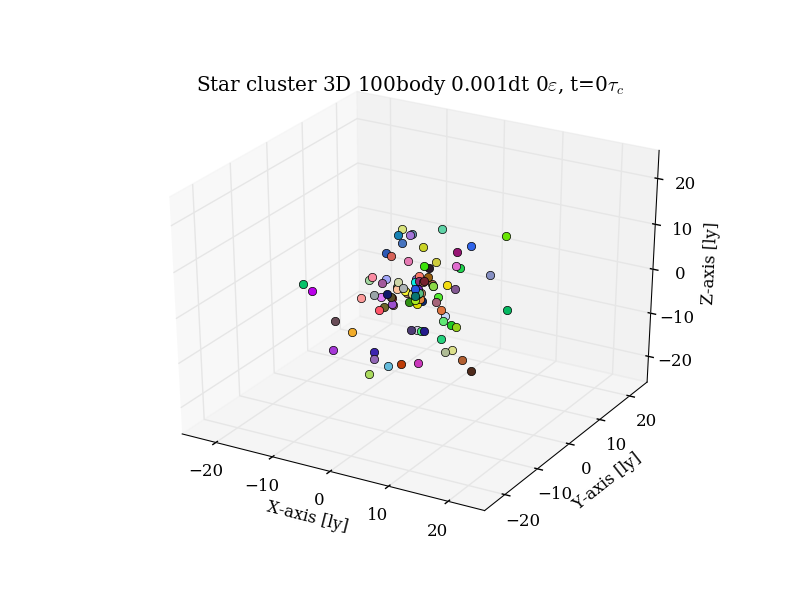
\includegraphics[scale=0.35]{../moviefigs/ClusterPos_100body_dt1_eps0_dur16_movie0.png}
\caption{$\mathbf{N} = 100$ body cluster simulation at $t = 0\tau_c$.}
\end{figure}
\begin{figure}
[H]\center
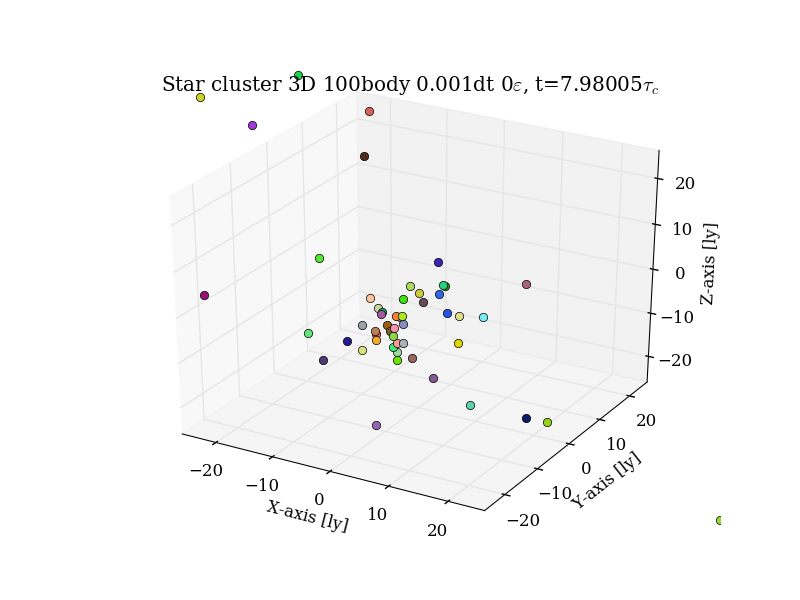
\includegraphics[scale=0.35]{../moviefigs/ClusterPos_100body_dt1_eps0_dur16_movie200.png}
\caption{$\mathbf{N} = 100$ body cluster simulation at $t \simeq 7.5\tau_c$.}
\end{figure}
\begin{figure}
[H]\center
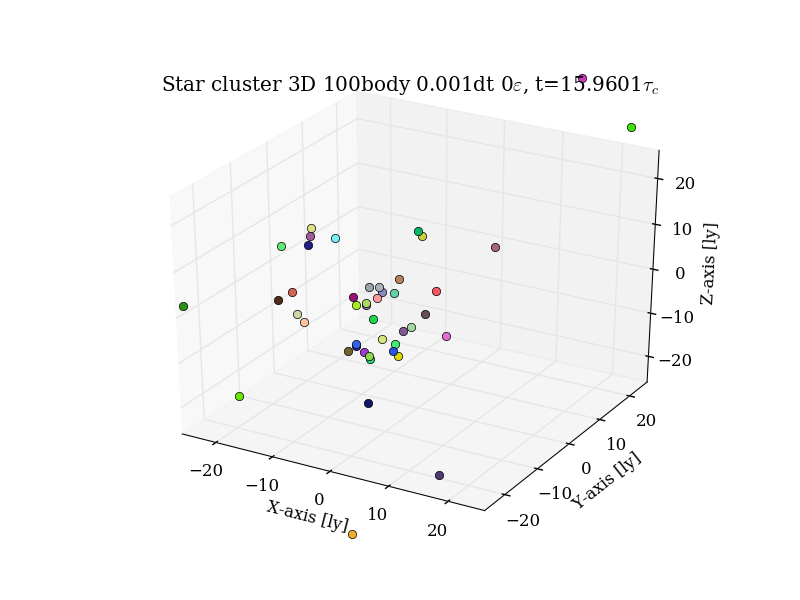
\includegraphics[scale=0.35]{../moviefigs/ClusterPos_100body_dt1_eps0_dur16_movie400.png}
\caption{$\mathbf{N} = 100$ body cluster simulation at $t \simeq 16\tau_c$.}
\end{figure}

Running the simulation for varying values of $N = 100, 200, 400$ yielded the following plots \newpage

\begin{figure}
[H]\center
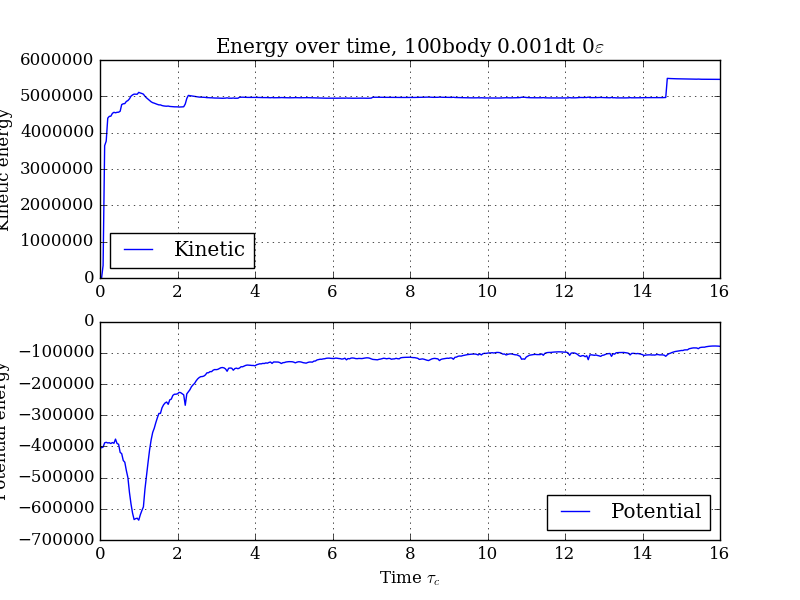
\includegraphics[scale=0.35]{../figs/ClusterEnergiesSys_100body_dt1_eps0_dur16.png}
\caption{$\mathbf{N} = 100$ body cluster's energy development, all bodies' energies summed for every time step, over a duration of $t \simeq 16\tau_c$.}\label{fig:N100eps0dur16energy}
\end{figure}
\begin{figure}
[H]\center
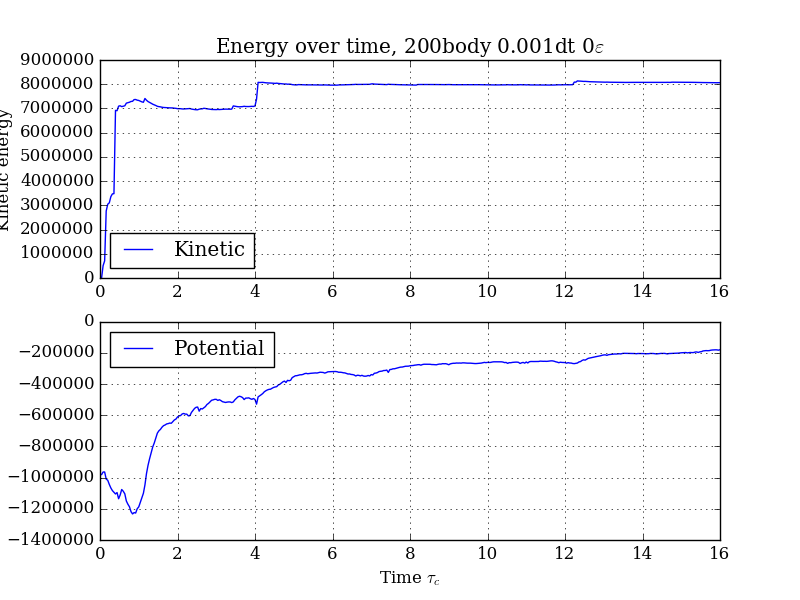
\includegraphics[scale=0.35]{../figs/ClusterEnergiesSys_200body_dt1_eps0_dur16.png}
\caption{$\mathbf{N} = 200$ body cluster's energy development, all bodies' energies summed for every time step, over a duration of $t \simeq 16\tau_c$.}
\label{fig:N200eps0dur16energy}
\end{figure}
\begin{figure}
[H]\center
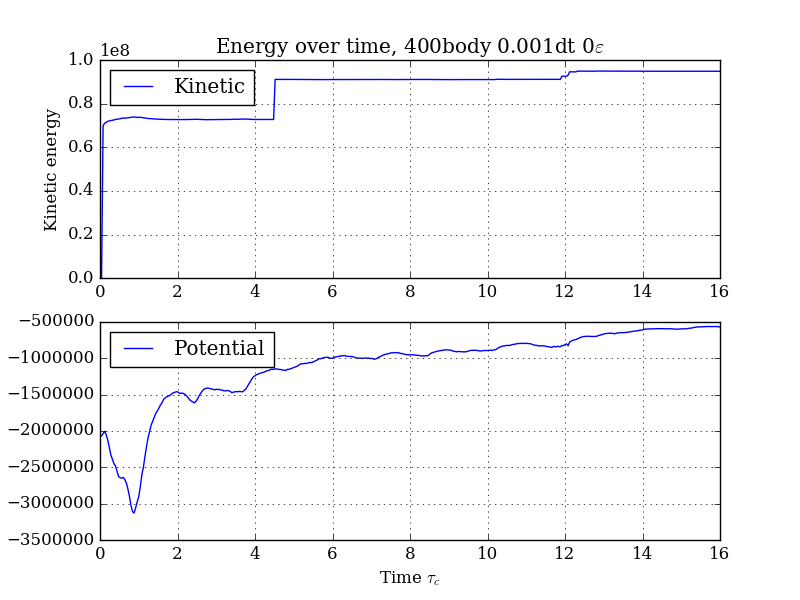
\includegraphics[scale=0.35]{../figs/ClusterEnergiesSys_400body_dt1_eps0_dur16.png}
\caption{$\mathbf{N} = 400$ body cluster's energy development, all bodies' energies summed for every time step, over a duration of $t \simeq 16\tau_c$.}
\label{fig:N400eps0dur16energy}
\end{figure}

\begin{figure}
[H]\center
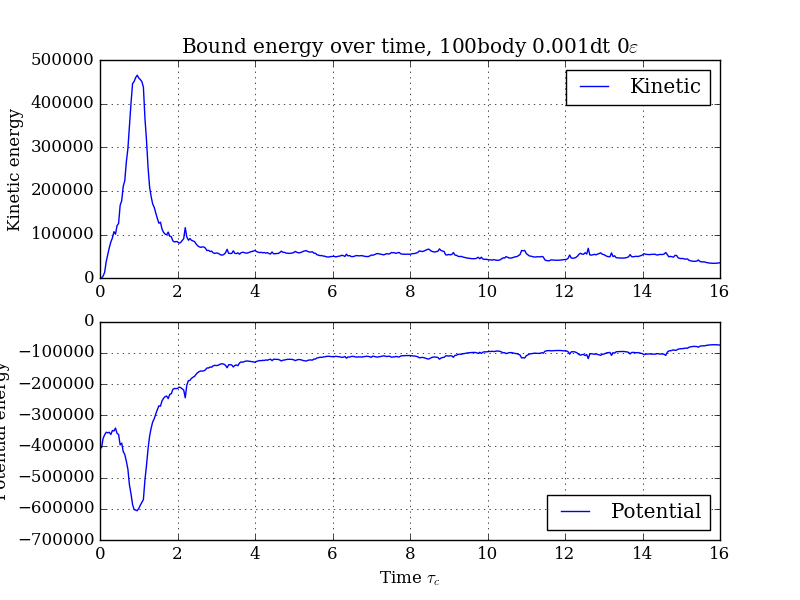
\includegraphics[scale=0.35]{../figs/ClusterEnergiesComp_100body_dt1_eps0_dur16.png}
\caption{$\mathbf{N} = 100$ \textit{bound} body cluster's energy development, all \textit{bound} bodies' energies summed for every time step.}
\end{figure}
\begin{figure}
[H]\center
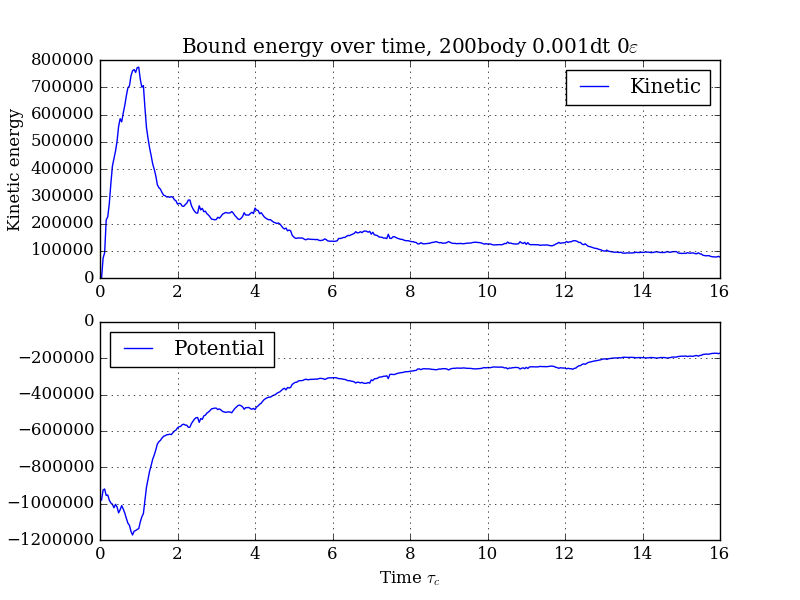
\includegraphics[scale=0.35]{../figs/ClusterEnergiesComp_200body_dt1_eps0_dur16.png}
\caption{$\mathbf{N} = 200$ \textit{bound} body cluster's energy development, all \textit{bound} bodies' energies summed for every time step.}
\end{figure}
\begin{figure}
[H]\center
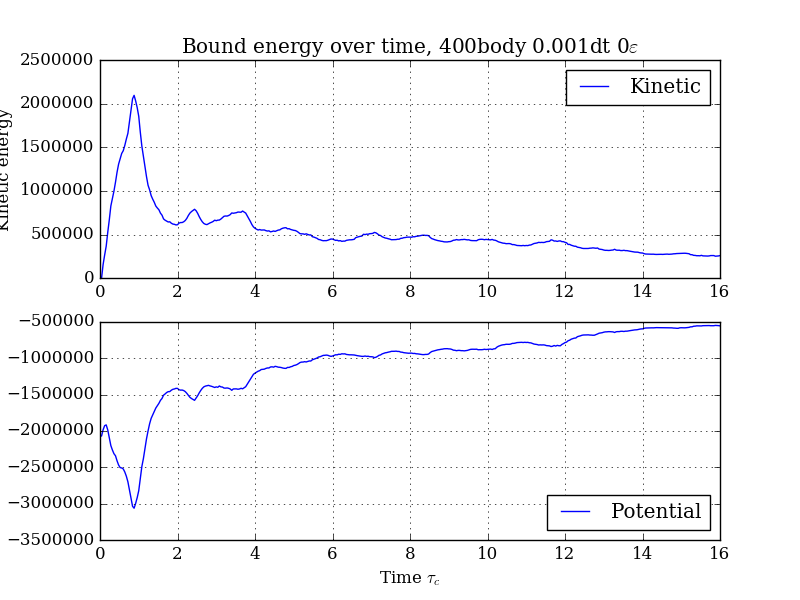
\includegraphics[scale=0.35]{../figs/ClusterEnergiesComp_400body_dt1_eps0_dur16.png}
\caption{$\mathbf{N} = 400$ \textit{bound} body cluster's energy development, all \textit{bound} bodies' energies summed for every time step.}
\end{figure}

\begin{figure}
[H]\center
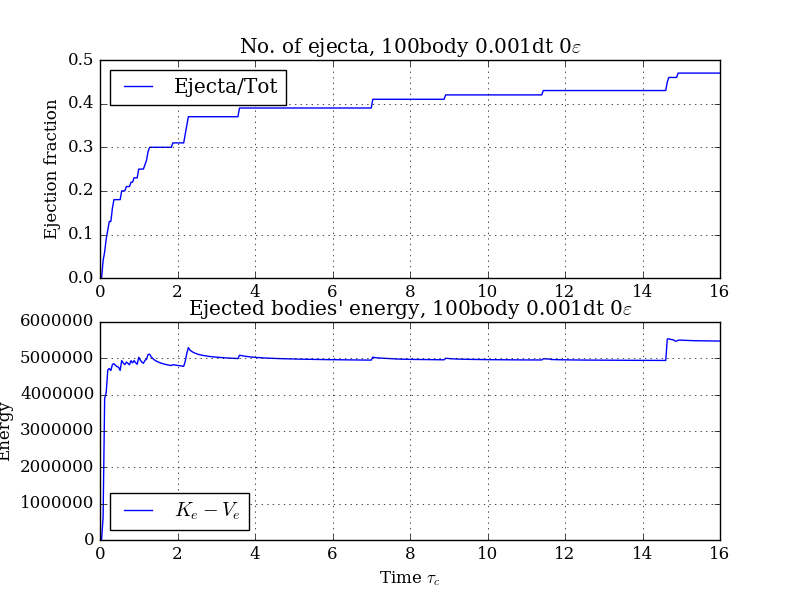
\includegraphics[scale=0.35]{../figs/ClusterEnergiesEjecEn_100body_dt1_eps0_dur16.png}
\caption{$\mathbf{N} = 100$ body cluster's ejected bodies' counting over a duration of $t \simeq 16\tau_c$, and energy of ejected bodies.}
\end{figure}
\begin{figure}
[H]\center
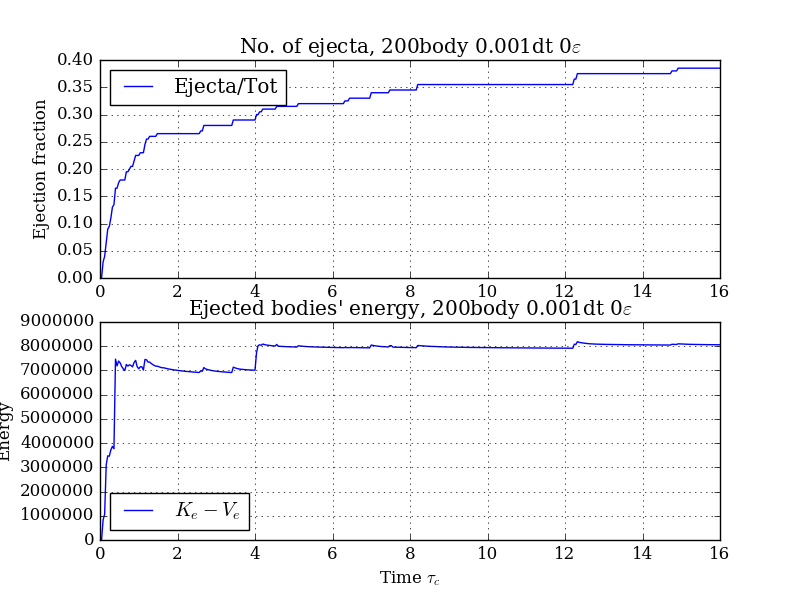
\includegraphics[scale=0.35]{../figs/ClusterEnergiesEjecEn_200body_dt1_eps0_dur16.png}
\caption{$\mathbf{N} = 200$ body cluster's ejected bodies' counting over a duration of $t \simeq 16\tau_c$, and energy of ejected bodies.}
\end{figure}
\begin{figure}
[H]\center
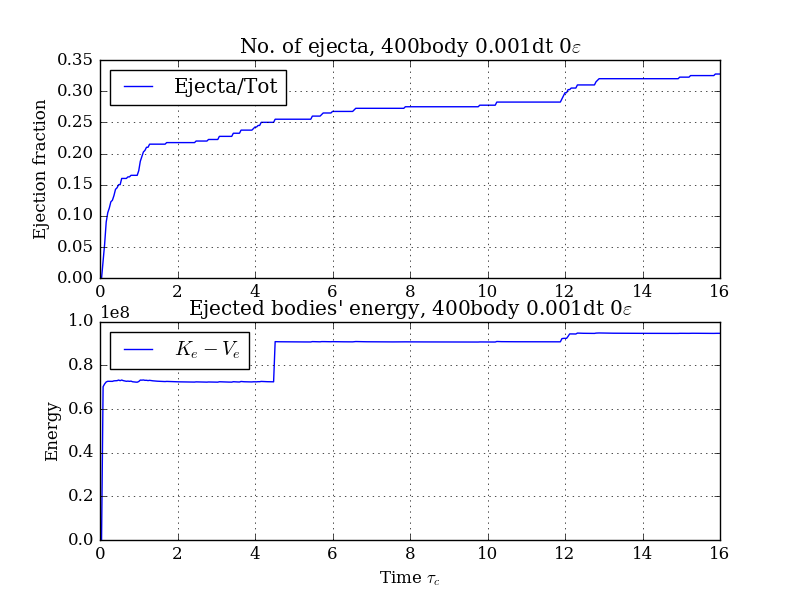
\includegraphics[scale=0.35]{../figs/ClusterEnergiesEjecEn_400body_dt1_eps0_dur16.png}
\caption{$\mathbf{N} = 400$ body cluster's ejected bodies' counting over a duration of $t \simeq 16\tau_c$, and energy of ejected bodies.}
\end{figure}

\begin{figure}
[H]\center
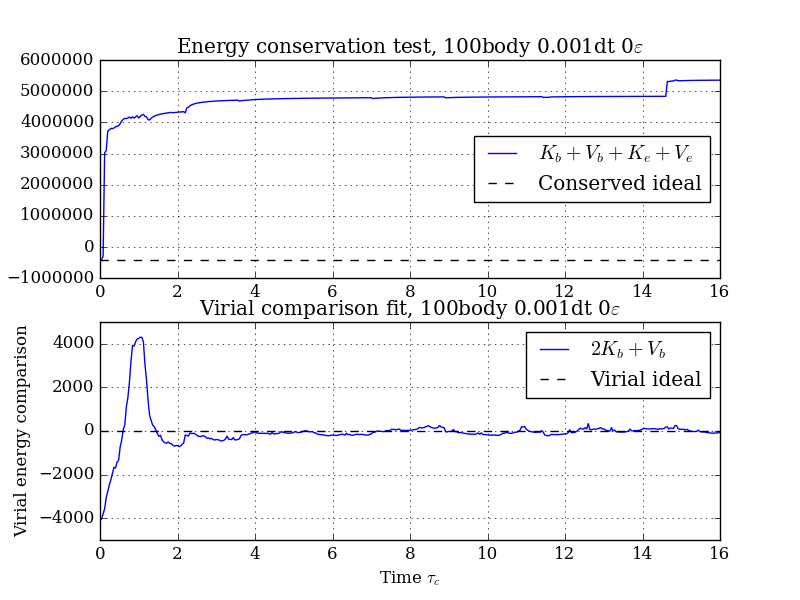
\includegraphics[scale=0.35]{../figs/ClusterEnConsvVirial_100body_dt1_eps0_dur16.png}
\caption{$\mathbf{N} = 100$ body cluster's energy conservation illustration and virial approximation, over a duration of $t \simeq 16\tau_c$.}\label{fig:N100eps0consVirial}
\end{figure}
\begin{figure}
[H]\center
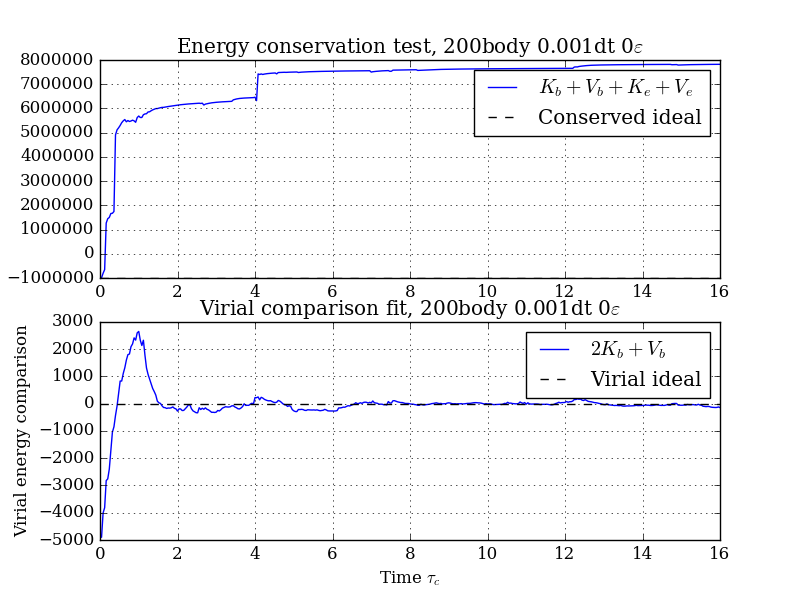
\includegraphics[scale=0.35]{../figs/ClusterEnConsvVirial_200body_dt1_eps0_dur16.png}
\caption{$\mathbf{N} = 200$ body cluster's energy conservation illustration and virial approximation, over a duration of $t \simeq 16\tau_c$.}
\label{fig:N200eps0consVirial}
\end{figure}
\begin{figure}
[H]\center
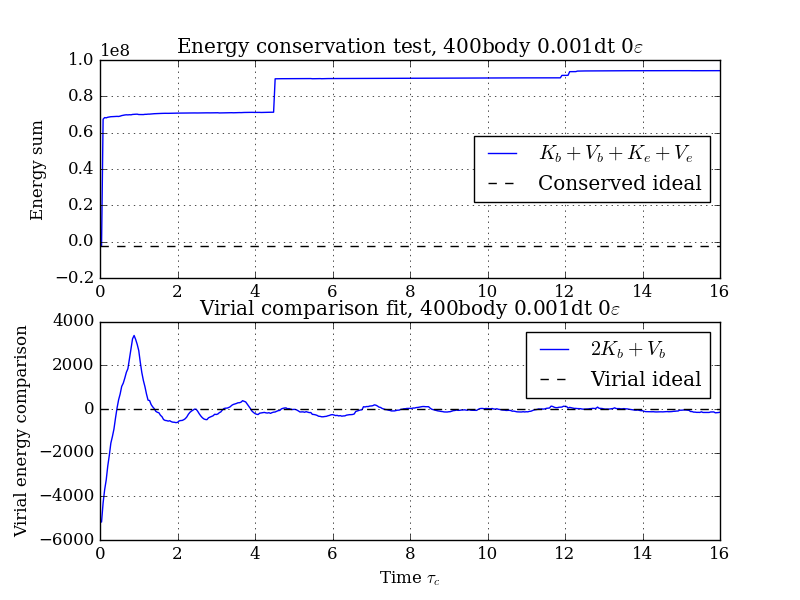
\includegraphics[scale=0.35]{../figs/ClusterEnConsvVirial_400body_dt1_eps0_dur16.png}
\caption{$\mathbf{N} = 400$ body cluster's energy conservation illustration and virial approximation, over a duration of $t \simeq 16\tau_c$.}
\label{fig:N400eps0consVirial}
\end{figure}

\subsection{Simulations without numerical round-off correction discussion}
Having seen the development of the cluster by plots and animation, it seems that the cluster almost immediately ejects some of its contents, and as the rest of the structure collapses, even more material is flung, the flinging being indicated by the sudden increases in kinetic energy from figure \ref{fig:N100eps0dur16energy}, sideways and beyond, at regular intervals when the stellar distribution seems to pulse with time.

It is clear that for no matter how long a duration one might choose run this set of initial conditions, a large fraction of stellar bodies are ejected and flung across space, effectively never to be bound by the cluster's gravitational potential well again.

One might consider the aforementioned apparent motion of pulsation to be the energies of the system reaching an equilibrium point, which is the ideal for a gravitationally bound system. However, as such a large quantity of bodies that initially belonged to the cluster are ejected, then this seems a poor equilibrium for the initial system - even though the remaining core bodies seem to waltz around peacefully enough.

In other words, whereas the system as a whole, with all bodies from the initial setup, is far from reaching an equilibrium state, the core that remains and continues to dance by the music of gravity, seems to reach some kind of near-equilibrium at a time around 2$\tau_c$, as indicated by the figures \ref{fig:N100eps0consVirial}, \ref{fig:N200eps0consVirial}, \ref{fig:N400eps0consVirial}, that show how the remaining bound bodies' energies seem to oscillate around viriality, as per the virial theorem and equation \ref{eq:virial}.

A question then arises, in relation to the ergodeic hypothesis, from which we declared that an average over the whole system would replace the time average, to calculate viriality: how large a system is large enough? This speaks to the fact that for $N = 100$, around half of the bodies are ejected, which is quite a large fraction of bodies to lose and take an average over.

However, as stated earlier, quite a lot of energy is lost to the system from the ejection that is due to numerical instabilities of the cluster's bodies' force exchange, and we see this clearly when looking at the magnitude scale of kinetic energies, which have been raised way beyond any measure of energy conservation, as per aforementioned figures \ref{fig:N100eps0consVirial}, \ref{fig:N200eps0consVirial}, \ref{fig:N400eps0consVirial}, and energy is then clearly not conserved in these simulations.

While the energy taken away from the system is clearly quite large to begin with, it also seems to scale with increasing factor $N$, in accordance with the sense that an increased number of bodies that might potentially be ejected, an increased number of bodies are indeed ejected, which means that the total amount of energy ejected is bigger. The fractional ejection trend, however, seems to decrease with increasing $N$ bodies.

One might then speculate that by a number of $N$ great enough, the fraction of ejected bodies might be so small, that even their collected energies will also be so small, that the simulational error which I will attempt to fix by introducing the modified gravity per equation \ref{eq:modgravlaw}, might not even be necessary in the great picture.

A counter-indication to this, is the fact that the count of ejected particles seem to increase slowly but steadily, even after an equilibrium has been reached.

\subsection{Finding numerical instability round-off correction constant results}
To find the best value for $\varepsilon$ as a numerical instability correction constant, simulations are for a range of $\varepsilon = 0.01, 0.1, 1$ respectively. Energy conservation, ejected bodies' count, and ejected kinetic energy is investigated.

\begin{figure}
[H]\center
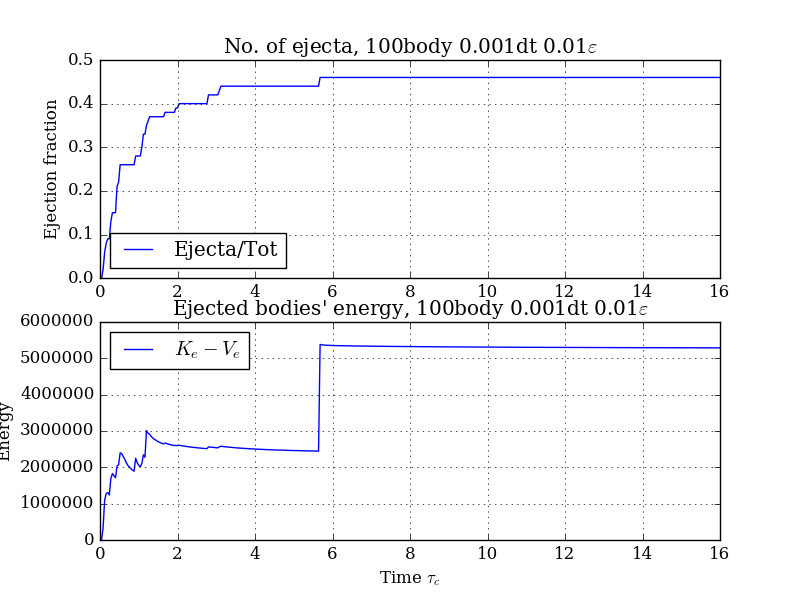
\includegraphics[scale=0.35]{../figs/ClusterEnergiesEjecEn_100body_dt1_eps1_dur16.png}
\caption{$\mathbf{N} = 100$ body cluster's ejected bodies' counting with $\varepsilon = 0.01$, and energy of ejected bodies.}\label{fig:N100eps1ejecEn}
\end{figure}
\begin{figure}
[H]\center
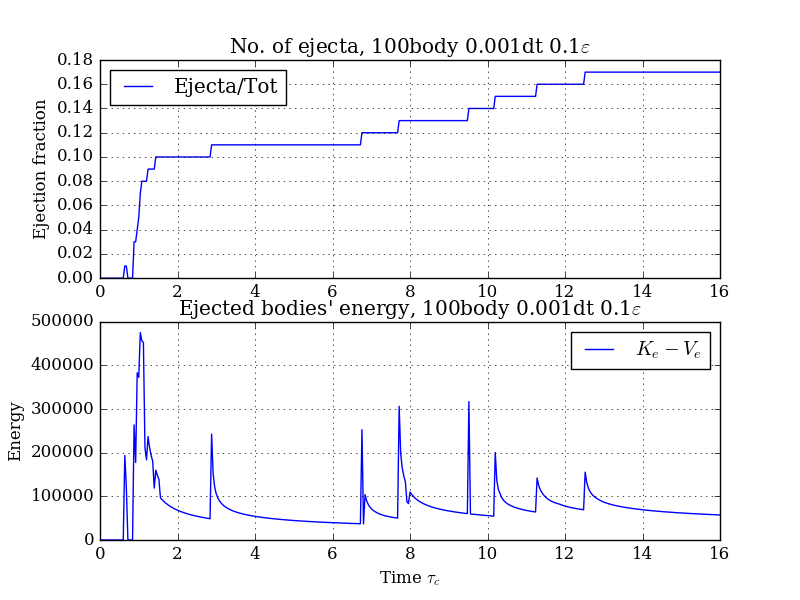
\includegraphics[scale=0.35]{../figs/ClusterEnergiesEjecEn_100body_dt1_eps10_dur16.png}
\caption{$\mathbf{N} = 100$ body cluster's ejected bodies' counting with $\varepsilon = 0.1$, and energy of ejected bodies.}\label{fig:N100eps10ejecEn}
\end{figure}
\begin{figure}
[H]\center
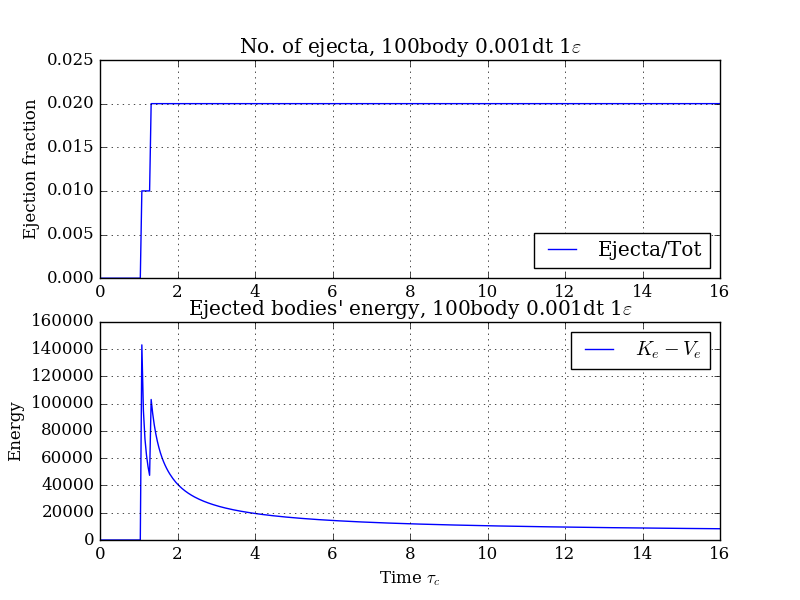
\includegraphics[scale=0.35]{../figs/ClusterEnergiesEjecEn_100body_dt1_eps100_dur16.png}
\caption{$\mathbf{N} = 100$ body cluster's ejected bodies' counting with $\varepsilon = 1$, and energy of ejected bodies.}\label{fig:N100eps100ejecEn}
\end{figure}

\begin{figure}
[H]\center
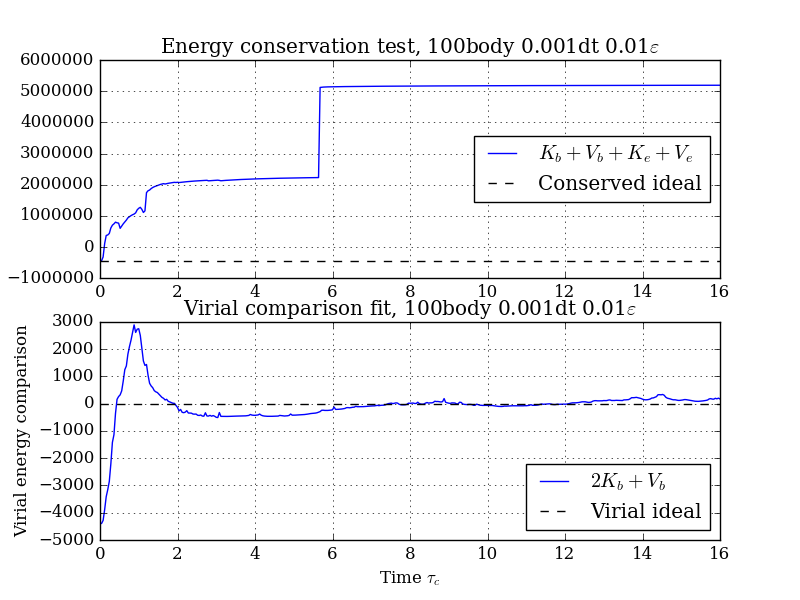
\includegraphics[scale=0.35]{../figs/ClusterEnConsvVirial_100body_dt1_eps1_dur16.png}
\caption{$\mathbf{N} = 100$ body cluster's energy conservation illustration and virial approximation, with $\varepsilon = 0.01$.}\label{fig:N100eps1consVirial}
\end{figure}
\begin{figure}
[H]\center
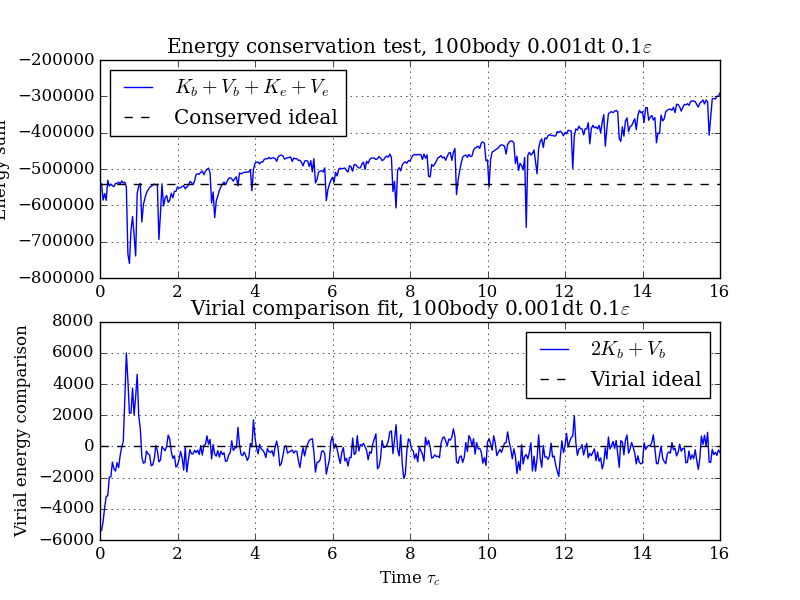
\includegraphics[scale=0.35]{../figs/ClusterEnConsvVirial_100body_dt1_eps10_dur16.png}
\caption{$\mathbf{N} = 100$ body cluster's energy conservation illustration and virial approximation, with $\varepsilon = 0.1$.}\label{fig:N100eps10consVirial}
\end{figure}
\begin{figure}
[H]\center
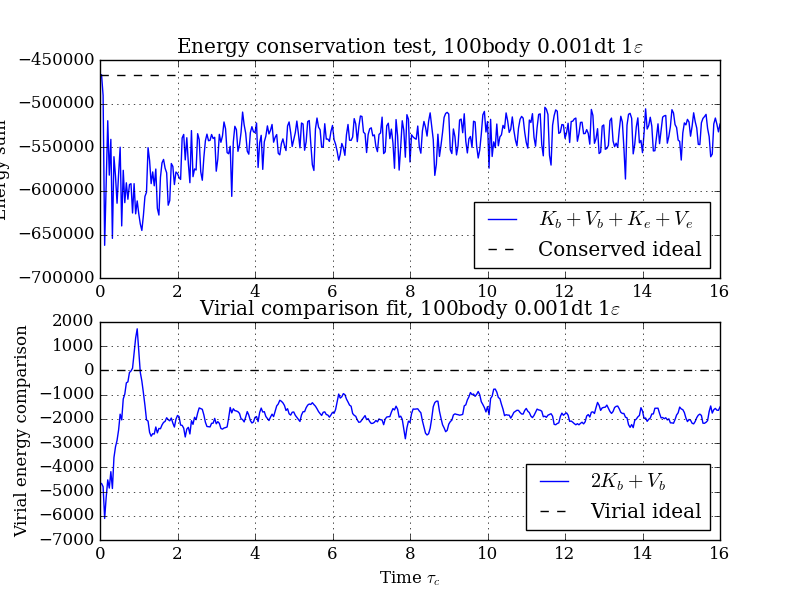
\includegraphics[scale=0.35]{../figs/ClusterEnConsvVirial_100body_dt1_eps100_dur16.png}
\caption{$\mathbf{N} = 100$ body cluster's energy conservation illustration and virial approximation, with $\varepsilon = 1$.}\label{fig:N100eps100consVirial}
\end{figure}

\subsection{Finding numerical instability round-off correction constant discussion}
The goal here is to reach a model, by using the gravity equation \ref{eq:modgravlaw}, which introduces the correction term $\varepsilon$, so that the final model has \begin{itemize}
\item as few as possible non-sensical kinetic energy spikes divided on a few bodies, to mantain physicality.
\item a final model in which the energy seems to be conserved in the system.
\item and where the system seems to virialize towards an equilibrium state.
\end{itemize}

The system should be free to eject bodies, as long as these bodies have reasonable kinetic energies, and total energy amount is conserved.

With $\varepsilon$ set to $\varepsilon = 0.01$, there are still seemingly non-physical spikes of energy, figure \ref{fig:N100eps1ejecEn}, long after the system of bodies have seemed to gravitationally virialize, figure \ref{fig:N100eps1consVirial}. The fraction of ejecta is also still quite high, figure \ref{fig:N100eps1ejecEn}, and energy is definitely not conserved, according to figure \ref{fig:N100eps1consVirial}.

For the other side of the range, $\varepsilon = 1$, very few objects are ejected, figure \ref{fig:N100eps100ejecEn}, and the kinetic energy spikes only happen a few times in the beginning, before these energies fade. On the other hand, both the energy conservation and the virialization belonging to this dataset is oscillating below ideal values, at great enough a magnitude that the data looks intuitively wrong. As discussed in section \ref{section:matheps}, this seems to indicate that the magnitude value of $\varepsilon = 1$ is too great to \textit{not} diffuse the macroscopic system's calculation.

Lastly, for the middle value of the investigated range of $\varepsilon$s, there is $\varepsilon = 0.1$. This set value of the round-off correction term yielded a fairly reasonably low magnitude of ejected bodies, and the largest spike in ejection energy does not seem unreasonable, figure \ref{fig:N100eps10ejecEn}. At the same time, the system's energy conservation level seems to hover nearby the ideal level - despite a some minor aberrations, figure \ref{fig:N100eps10consVirial}.

In this figure it is also seen how the energy seems the closest to being conserved around the time mark $\tau_c = 5$, although at times after this mark, the sum of the known energies seems set on a positive slope for no good reason. This is likely because the numerical instability correction term, $\varepsilon$, while used in the force exchange equation \ref{eq:modgravlaw}, is not taken account for in the potential energy equation \ref{eq:PotEn}.

So wherein I have discovered that a value for the round-off correction term $\varepsilon = 0.1$ might be a good value, it is not a perfect value, or even a perfect solution, and simulated $N$-body systems' physicality could be speculated to become more and more unphysical after a time frame of $\tau_c = 5$, or $\tau_c = 6$.

\subsection{Radial density results}
Choosing equilibrium time to be around $t \simeq 4.5\tau_c$, these plots of radial distribution are retrieved from the data.
\begin{figure}
[H]\center
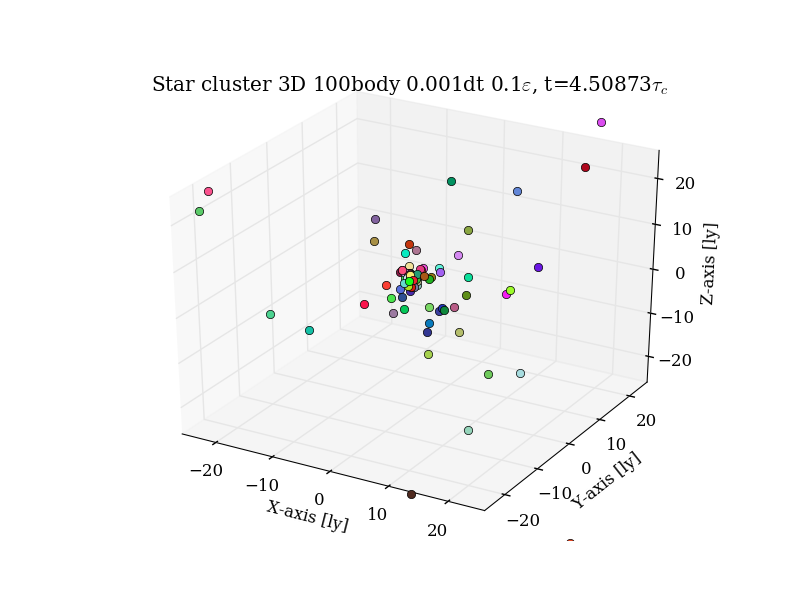
\includegraphics[scale=0.35]{../moviefigs/eps10/ClusterPos_100body_dt1_eps10_dur16_movie113.png}
\caption{$\mathbf{N} = 100$ body cluster simulation at $t \simeq 4.5\tau_c$.}\label{fig:N100eps10eq}
\end{figure}
\begin{figure}
[H]\center
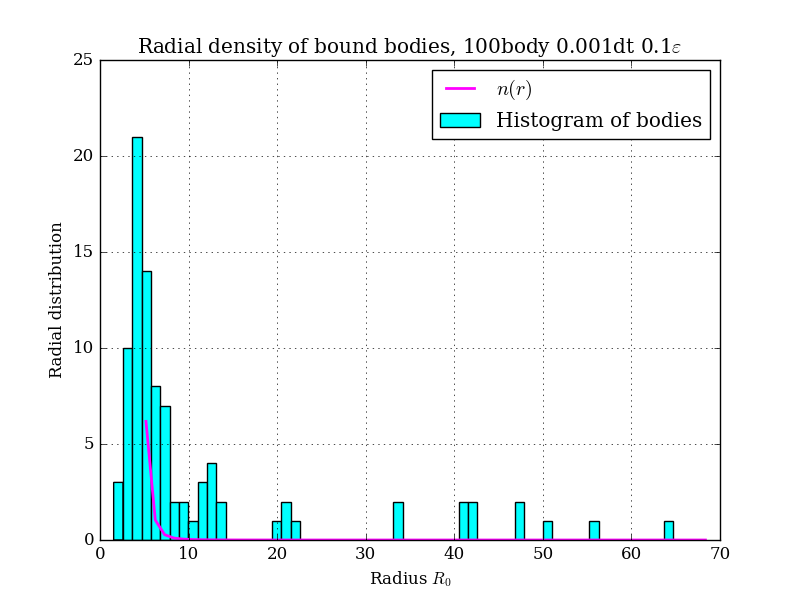
\includegraphics[scale=0.35]{../figs/ClusterRadDens_100body_dt1_eps10_dur16.png}
\caption{$\mathbf{N} = 100$ body cluster simulation at $t \simeq 4.5\tau_c$.}\label{fig:N100eps10eqHist}
\end{figure}

\subsection{Radial density discussion}

\section{Appendix}
\subsection{Code and GitHub}
All my code is located at this address:

\url{https://github.com/magnucb/p5}

\begin{thebibliography}{9}
\bibitem{example_code}
  Jensen, M 2016,
  
  \verb|CodeName|,
  
  viewed $9^{th}$ of December 2016,
  
  \url{URL}

\bibitem{cold_collapse}
	M. Joyce, B. Marcos, and F. Sylos Labini 2010,
	
	Cold uniform spherical collapse revisited
	
	viewed $9^{th}$ of December 2016,
		
	\url{https://arxiv.org/pdf/1011.0614v1.pdf}
	
\bibitem{STHM}
	M. Dijkstra,
	
	AST4320: Cosmology and Extragalactic Astrophysics,
	
	viewed $^{th}$ of December 2016,
	
	\url{https://dl.dropboxusercontent.com/u/16515147/AST4320/LecturenotesAST4320_Nov30.pdf}
\end{thebibliography}

\end{document}